\section{MOS Transistoren}

\subsection{Dotierung}
\begin{center}
    \begin{tabular}{lll}
        \textbf{Dotierung:}          & N-dotiert            & P-dotiert \\
        \textbf{Unreinheit:}         & Aluminium (HG III)   & Phosphor / Arsen (HG V) \\
        \textbf{Majoritätsträger:}   & Elektronen           & Löcher \\
        \textbf{Minoritätsträger:}   & Löcher               & Elektronen \\
    \end{tabular}
\end{center}


\subsection{MOS-Kapazität}
\begin{minipage}[t]{0.5\columnwidth}
    Minoritätsträger werden an das Gate gezogen.
    Die entstandene Raumladungszone weist bei ausreichend hoher Gate-Spannung einen Minoritätsträgerüberschuss auf, ist also in der Funktion \textbf{komplementär} zum Substrat dotiert.
\end{minipage}
\hfill
\begin{minipage}[t]{0.48\columnwidth}
    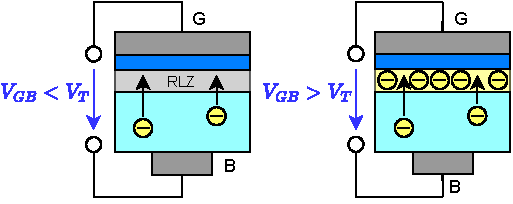
\includegraphics[width=\columnwidth, align=t]{images/02_MOS_kapazitaet.pdf}
\end{minipage}


\subsection{MOS-Transistoren}
Werden links und rechts vom MOS-Kondensator komplementär zum Substrat dotierte Regionen (Drain und Source) erstellt, so kann ohne Gatespannung aufgrund der PN-Übergänge kein Strom vom Drain zur Source (oder umgekehrt) fliessen.
Wird nun eine Spannung am Gate angelegt, so entsteht die Minoritätsträger-Leitende Raumladungszone - der Kanal.
Dieser verbindet Drain und Source, es kann also ein Strom fliessen.

\vspace{-0.2cm}

\begin{center}
    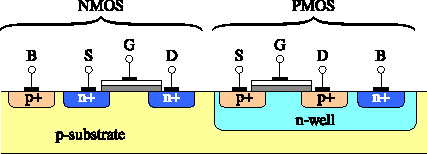
\includegraphics[width=0.5\columnwidth, align=t]{images/02_CMOS.pdf}
\end{center}


\subsubsection{Übersicht und Symbole}

\begin{minipage}[t]{0.48\columnwidth}
    Durch Vordotierung des Kanals kann der Transistor ohne Gate-Spannung leitend gemacht werden (Verarmungstyp, selbstleitend).
    Eine negative Gate-Spannung kann den Kanal dann abschnüren. \\
    \rightarrow\ hier nicht weiter behandelt

    \smallskip

    \textbf{Der Bulk wird nur eingezeichnet, wenn dieser \myul{nicht} mit $\bm{V_{\rm DD}}$ bzw. $\bm{V_{\rm SS}}$ verbunden ist.}
    Deshalb werden meist die vereinfachten Symbole verwendet:

    \vspace{-0.3cm}

    \begin{center}
        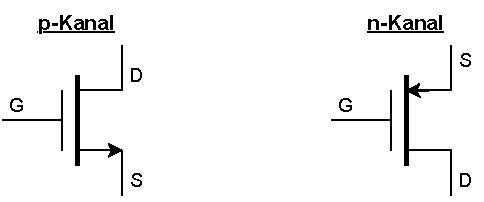
\includegraphics[width=0.8\columnwidth, align=t]{images/02_MOSFET_symbole_vereinfacht.pdf}
    \end{center}
\end{minipage}
\hfill
\begin{minipage}[t]{0.5\columnwidth}
    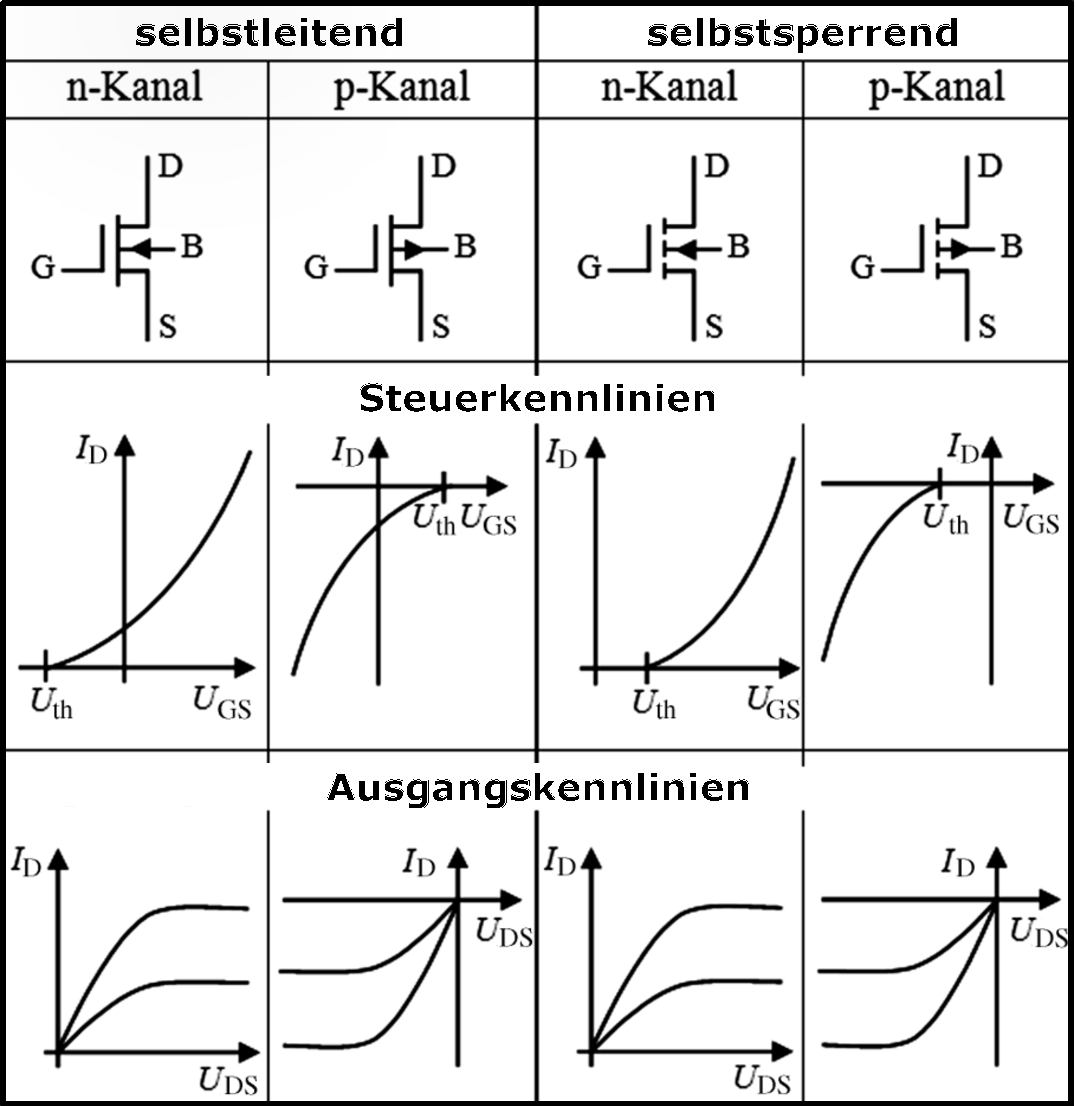
\includegraphics[width=\columnwidth, align=t]{images/02_MOSFET_uebersicht.pdf}
\end{minipage}



\subsubsection{Modelle}
In Cadence sind verschiedene Modelle hinterlegt:

\textbf{Spice Modell 11:} Das Modell 11 beinhaltet ca. 100 Parameter und ist entsprechend genau.

\textbf{Spice Modell 1:} Vergleichbar mit dem Handrechenmodell, welches zwar weniger genau, dafür aber viel einfacher ist. Dennoch beinhaltet es bereits 40 Parameter.

\subsection{Ausgangskennlinie -- Arbeitsbereiche}
 
Die Ausgangskennlinie beschreibt den Zusammenhang $I_D = f(V_{DS}) \big|_{V_{GS} = \text{konst}}$

\begin{minipage}[t]{0.5\columnwidth}
    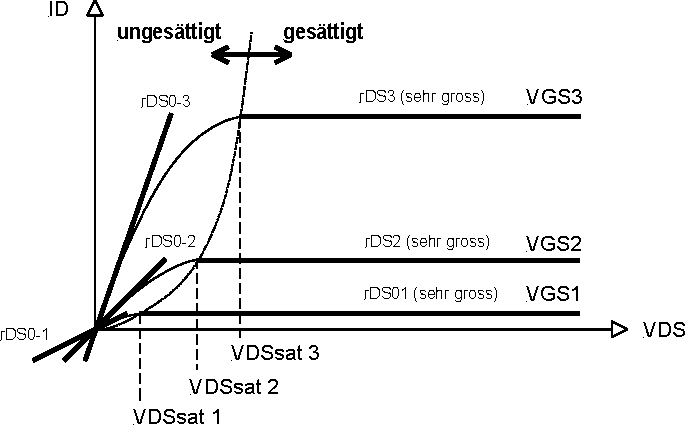
\includegraphics[width=\columnwidth, align=t]{images/02_MOSFET_ausgangskennlinien.pdf}
\end{minipage}
\hfill
\begin{minipage}[t]{0.48\columnwidth}
    Zwei Arbeitsbereiche: 

    \begin{outline}
        \1 ungesättig (gesteuerter Widerstand)
        \1 gesättigt (Stromquelle)
    \end{outline}

    \medskip

    Die Sättigungsgrenze $V_{\rm DS, sat}$ ist abhängig vom \textbf{Kanalzustand}:

    \begin{outline}
        \1 \textbf{weak inversion:} \\
            $V_{\rm DS, sat} = V_{\rm eff} \approx 5 \cdot V_{\rm temp} \approx \qty{130}{\milli \volt}$ 
        \1 \textbf{strong inversion:} \\
            $V_{\rm DS, sat} = V_{\rm eff} = V_{GS} - V_T$ 
    \end{outline}
\end{minipage}



\subsection{Transferkennlinie -- Ausgangsstrombereiche}


\begin{minipage}[t]{0.55\columnwidth}
    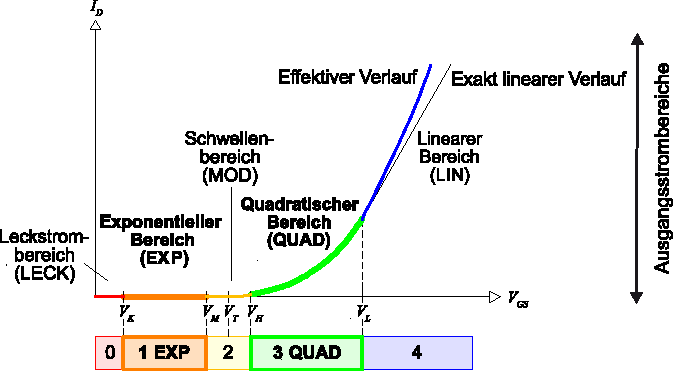
\includegraphics[width=\columnwidth, align=t]{images/02_MOSFET_transferkennlinie.pdf}
\end{minipage}
\hfill
\begin{minipage}[t]{0.42\columnwidth}
    Die Transferkennlinie beschreibt den Zusammenhang $I_D = f(V_{GS})$ 

    \smallskip

    Dabei werden \textbf{5 Ausgangsstombereiche} unterschieden. Diese hängen mit dem \textbf{Kanalzustand} zusammen.

    \smallskip

    Des Weiteren gibt es die Bereiche:

    \begin{outline}
        \1 Sub Threshold: $V_{GS} < V_T$
        \1 Above Threshold: $V_{GS} > V_T$
    \end{outline}
\end{minipage}


\para{Ausgangsstrombereiche}

\scalebox{0.8}{
\begin{tabular}{|l|l|l|}
    \hline
    \textbf{Bereich}                    & \textbf{Mathem. Charakterisierung}            & \textbf{Zugrundeliegender phys. Effekt}                       \\  
    \hline
    \rowcolor[HTML]{F4CCCC} 
    LECK                                & $I_D$ erreicht Minimalwert, der nicht         & Drain- und Source-Substratdiode haben                         \\
    \rowcolor[HTML]{F4CCCC} 
                                        & weiter unterschritten werden kann             & Leckströme ins Subsstrat                                      \\
    \hline
    \rowcolor[HTML]{FFE5BB} 
    EXP                                 & $I_D$ steigt exponentiell mit $V_{GS}$        & Kanal zeigt \textbf{weak inversion}                           \\
    \hline
    \rowcolor[HTML]{FFF2CC} 
    MOD                                 & Keine 'handliche' Formel für $I_D$            & Kanal zeigt \textbf{moderate inversion}                       \\
    \hline
    \rowcolor[HTML]{D9EAD3} 
    QUAD                                & $I_D$ steigt quadratisch mit $V_{GS}$         & Kanal zeigt \textbf{strong inversion}                         \\
    \hline
    \rowcolor[HTML]{CFE2F3} 
    LIN                                 & $I_D$ steigt annähernd linear mit $V_{GS}$    & Geschwindigkeitssättigung der Ladungsträger im Kanal          \\
    \rowcolor[HTML]{CFE2F3} 
                                        & (halb QUAD, halb LIN)                         & im Kanal (nicht weiter beschleunigbar)                        \\
    \hline
\end{tabular}
}

\smallskip

\textbf{Hinweis:} Die Inversion des Kanals beschreibt, wie sehr sich die Polarität geändert ('invertiert') hat. 
Bei einem n-Kanal FET ist der Kanal ursprünglich p-leidend.
Wird der Kanal invertiert, so wird er (schwach, moderat oder start) n-leitend. 

%NOTE [Simi] Kommt später bei Pi-Ersatzschaltung verallgemeinert dran und ist daher hier auskommentiert
% \subsection{Ersatzschaltungen}

% Je nach Arbeitsbereich (gesättigt / ungesättigt) müssen verschiedene Ersatzschaltungen verwendet werden.

% \begin{minipage}[t]{0.48\columnwidth}
%     \raggedright

%     \subsubsection*{Ungesättigt}

%     Gesteuerter Widerstand \rightarrow\ $I_D = f(V_{DS})$
    
%     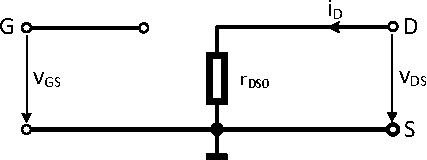
\includegraphics[width=\columnwidth, align=t]{images/02_MOSFET_ersatzschaltung_ungesaettigt.pdf}

%     \smallskip
%     Je kleiner $r_{\rm DS0}$, desto steiler die Geraden links im Ausgangskennlinienfeld

% \end{minipage}
% \hfill
% \begin{minipage}[t]{0.48\columnwidth}
%     \raggedright

%     \subsubsection*{Gesättigt}

%     Stromquelle \rightarrow\ $I_D = f(V_{GS})$

%     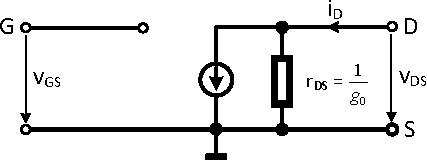
\includegraphics[width=\columnwidth, align=t]{images/02_MOSFET_ersatzschaltung_gesaettigt.pdf}

%     \smallskip
%     Je grösser $r_{\rm DS}$, desto flacher die Geraden rechts im Ausgangskennlinienfeld
% \end{minipage}


\subsection{Berechnung des Drainstroms}

Die Berechnung des Drainstroms hängt sowohl von Arbeitsbereich (gesättigt / ungesättig), als auch vom Ausgangsstrombereich (bzw. der Kanaliversion) ab!


\subsubsection{Strong Inversion}
\label{Strong Inversion}

\vspace{-0.3cm}

% $$ \boxed{ \text{QUAD-Bereich: } V_H(I_D) < V_{GS} < V_L(I_D) } \qquad \qquad \beta = \mu \cdot C_{\text{OX}} \cdot \frac{W}{L} $$
\[ \boxed{ \text{QUAD-Bereich:} \quad |V_H(I_D)| \leq |V_{GS}| < |V_L(I_D)| \quad \text{bzw.} \quad |I_H'| \leq |I_D'| < |I_L'| } \]  %NOTE: Bedingung für Ströme aus Ü3, 3.6.4 1)

\resizebox{\columnwidth}{!}
{
    \renewcommand{\arraystretch}{1.5}
    \begin{tabular}{@{}l c | c@{}}
                & \textbf{Ungesättigt:} \quad $\bm{| V_{DS} | < | V_{GS} - V_T |}$                                                              & \textbf{Gesättigt:} \quad $\bm{| V_{DS} | \geq | V_{GS} - V_T |}$                         \\
        NMOS:   & $I_D = \beta \cdot \bigg[ (V_{GS} - V_T) V_{DS} - \frac{V_{DS}^2}{2} \bigg] \cbl{\cdot (1 + \lambda \cdot \Delta V_{DS})}$    & $I_D = \frac{\beta}{2} (V_{GS} - V_T)^2 \cbl{\cdot (1 + \lambda \cdot \Delta V_{DS})}$    \\
        \midrule
        PMOS:   & $I_D = - \beta \cdot \bigg[ (V_{GS} - V_T) V_{DS} - \frac{V_{DS}^2}{2} \bigg] \cbl{\cdot (1 - \lambda \cdot \Delta V_{DS})}$  & $I_{D} = - \frac{\beta}{2} (V_{GS} - V_T)^2 \cbl{\cdot (1 - \lambda \cdot \Delta V_{DS})}$
    \end{tabular}
    \renewcommand{\arraystretch}{1}
}

\medskip

\textbf{Ohne} Berücksichtigung der \textbf{Kanallängenmodulation:} \cbl{blauen Term $=1$} bzw $\lambda = 0$ setzen



% NOTE [Simi] @Flurin: Hier noch dein Vorschlag der Darstellung (mit NMOS / PMOS Ergänzung):
% Jetzt können wir streiten, welchen wir nehmen wollen :P

% \resizebox{\columnwidth}{!}
% {
%     \renewcommand{\arraystretch}{1.5}
%     \begin{tabular}{l c|c}
%                 & \textbf{Ungesättigt:} \quad $\bm{| V_{\rm DS} | < | V_{GS} - V_T |}$                          & \textbf{Gesättigt:} \quad $\bm{| V_{\rm DS} | \geq | V_{GS} - V_T |}$             \\
%         NMOS:   & $I_{\rm D, ideal} = \beta \cdot \bigg[ (V_{GS} - V_T) V_{DS} - \frac{V_{DS}^2}{2} \bigg]$     & $I_{\rm D, ideal} = \frac{\beta}{2} (V_{GS} - V_T)^2 $                            \\
%         NMOS:   & $I_{\rm D, real} = I_{\rm D, ideal} \cdot (1 + \lambda \cdot \Delta V_{DS})$                  & $I_{\rm D, real} = I_{\rm D, ideal} \cdot (1 + \lambda \cdot \Delta V_{DS})$      \\
%         \midrule
%         PMOS:   & $I_{\rm D, ideal} = - \beta \cdot \bigg[ (V_{GS} - V_T) V_{DS} - \frac{V_{DS}^2}{2} \bigg]$   & $I_{\rm D, ideal} = - \frac{\beta}{2} (V_{GS} - V_T)^2$                           \\
%         PMOS:   & $I_{\rm D, real} = I_{\rm D, ideal} \cdot (1 - \lambda \cdot \Delta V_{DS})$                  & $I_{\rm D, real} = I_{\rm D, ideal} \cdot (1 - \lambda \cdot \Delta V_{DS})$      
%     \end{tabular}
%     \renewcommand{\arraystretch}{1}
% }



\paragraph{Transkonduktanz-Parameter $\bm{\beta}$}

\begin{minipage}[c]{0.78\columnwidth}
    $\beta$ ist abhängig davon, ob der Transistor gesättigt ist. 
    In der Praxis wird diese Unterscheidung jedoch \textbf{nicht} gemacht. 
    Im \textbf{Design} kann $\beta$ durch das Verhältnis von Kanalbreite $W$ und -länge $L$ beeinflusst werden.
\end{minipage}
\hfill
\begin{minipage}[c]{0.2\columnwidth}
    \[ \beta = \underbrace{ \mu C_{\rm OX} }_{\beta_0} \frac{W}{L} \]
\end{minipage}


%TODO: [Flurin] NMOSI und PMOSI V2S12
% NOTE: [Simi] @ Flurin: Bist du sicher, dass du diese Slide meinst...? 



%TODO: [Flurin] V3S9 nochmal studieren, macht iwie noch nicht so sinn.
\paragraph{Kanallängenmodulation $\bm{\lambda$} und Early-Spannung $\bm{V_E}$}

% Die Early-Spannung $V_E = a_E \cdot L$ setzt sich zusammen aus dem technologieabhängigen Early-Faktor $a_E$ und der Kanallänge $L$.
Die Kanallängenmodulation beschreibt die Nichtidealität der spannungsgesteurten Stromquelle (im Sättigungsbetrieb).

$$ \lambda = \frac{1}{V_E + V_{DS, \rm sat}} \approx \frac{1}{V_E} \approx \frac{1}{a_E \cdot L} \qquad \text{Idealfall: } \lambda = 0 \text{ \rightarrow\ } L = \infty $$ 

\textbf{Achtung:} $\bm{V_E}$ ist typischerweise negativ, wird jedoch \textbf{immer positiv angegeben}. 
Grafisch entspricht $V_E$ der Spannung $V_{DS}$, bei welcher die Verlängerung der Ausgangskennlinie (Sättigung) die $V_{DS}$-Achse schneidet.


%CHECK: [Flurin] Ich finde die Herleitung aus V3S9 überflüssig. Evtl. macht die Grafik zur Early-Spannung sinn? Braucht halt viel platz...
% [Simi] @Flurin: Ja, auf die Herleitung würde ich auch verzichten. Das Bild wäre allenfalls sinnvoll. 
% Aus Platzgründen habe ich etws 'Prosa' zur Early-Spannung geschrieben... Wirklich toll ist der Text aber auch nicht...


\paragraph{Body-Effekt}
Der Body-Effekt beschreibt die \textbf{Abhängigkeit der Schwellenspannung} $\bm{V_T}$ von der Source-Bulk-Spannung $V_{SB}$ als
\[ 
    V_T = V_{T0} \pm \Delta V_T 
    \quad \text{mit} \quad 
    \Delta V_T = \gamma\left(\sqrt{\abs{V_{SB}} + \abs{2\Phi_F}}-\sqrt{\abs{2\Phi_F}}\right)
\]

\rightarrow\ \textbf{Body-Effekt nur wirksam, wenn} $\mathbf{V_{SB} \neq \qty{0}{\volt}}$ \\
\rightarrow\ Reminder: Bulk nur gezeichnet, wenn nicht auf $V_{DD}$ oder $V_{SS}$

\medskip

Das Fermi-Potential $\Phi_F$ ist prozess- wie auch temperaturabhängig. Zudem ist es abhängig von der Dotierungsstärke.

%NOTE: [Simi] Wenn kein Platz: folgende Tabelle weglassen (diese Formeln sind uns gemäss Zbinden egal)
\begin{minipage}[c]{0.3\columnwidth}
    \[ \Phi_F = \frac{kT}{q} \ln \left( \frac{N_A}{n_i} \right) \]
    \[ \gamma_N \overset{n-Dotierung}{\approx} \qty{1.46}{\sqrt{\volt}} \]
    \[ \gamma_P \overset{p-Dotierung}{\approx} \qty{1.08}{\sqrt{\volt}} \]
\end{minipage}
\hfill
\begin{minipage}[c]{0.68\columnwidth}
    \begin{tabular}{rl}
        $n_i$       & Intrinsische ladungsdichte von Silizium   \\
        $N_A$       & Ladungsdichte der Akzeptoren              \\
        $\gamma$    & Body-Effekt-Konstante                     \\
        $T$         & \textbf{Absolute} Temperatur              \\
        $k$         & Boltzmann-Konstante $\qty{1.380649 e-23}{\joule\per\kelvin}$  \\
        $q$         & Elementarladung $\qty{1.602 e-19}{\coulomb}$
    \end{tabular}
\end{minipage}


\subsubsection{Weak Inversion}

\vspace{-0.3cm}

% $$ \boxed{ \text{EXP-Bereich: } V_K(I_D) < V_{GS} < V_M(I_D) \qquad \qquad V_M(I_D) = V_T(I_D) - x_M(I_D) } $$
\[ \boxed{ \text{EXP-Bereich: } |V_K(I_D)| < |V_{GS}| \leq |V_M(I_D)| \quad \text{bzw.} \quad |I_K'| < |I_D'| \leq |I_M'| } \]  %NOTE: Bedingung für Ströme aus Ü3, 3.6.5 1)


\resizebox{\columnwidth}{!}
{
    \renewcommand{\arraystretch}{1.5}
    \begin{tabular}{@{}l c | c@{}}
                & \textbf{Ungesättigt:} \quad $\bm{| V_{DS} | < | V_{GS} - V_T |}$                                                                                                  & \textbf{Gesättigt:} \quad $\bm{| V_{DS} | \geq | V_{GS} - V_T |}$                                                     \\
        NMOS:   & $I_D = I_M \cdot \e^{\frac{V_{GS} - V_M}{n_M \cdot V_\text{temp}}} \cdot (1 - \e^{-\frac{V_{DS}}{V_\text{temp}}}) \cbl{\cdot (1 + \lambda \cdot \Delta V_{DS})}$  & $I_D = I_M \cdot \e^{\frac{V_{GS} - V_M}{n_M \cdot V_\text{temp}}} \cbl{\cdot (1 + \lambda \cdot \Delta V_{DS})}$     \\
        \midrule
        PMOS:   & $I_D = I_M \cdot \e^{- \frac{V_{GS} - V_M}{n_M \cdot V_\text{temp}}} \cdot (1 - \e^{\frac{V_{DS}}{V_\text{temp}}}) \cbl{\cdot (1 - \lambda \cdot \Delta V_{DS})}$ & $I_D = I_M \cdot \e^{- \frac{V_{GS} - V_M}{n_M \cdot V_\text{temp}}} \cbl{\cdot (1 - \lambda \cdot \Delta V_{DS})}$   \\
    \end{tabular}
    \renewcommand{\arraystretch}{1}
}

\medskip

\textbf{Ohne} Berücksichtigung der \textbf{Kanallängenmodulation:} \cbl{blauen Term $=1$} bzw $\lambda = 0$ setzen





% NOTE [Simi] @Flurin: Hier noch dein Vorschlag der Darstellung (mit NMOS / PMOS Ergänzung):
% Jetzt können wir streiten, welchen wir nehmen wollen :P

% \resizebox{\columnwidth}{!}
% {
%     \renewcommand{\arraystretch}{1.5}
%     \begin{tabular}{l c|c}
%                 & \textbf{Ungesättigt:} \quad $\bm{| V_{\rm DS} | < | V_{GS} - V_T |}$                          & \textbf{Gesättigt:} \quad $\bm{| V_{\rm DS} | \geq | V_{GS} - V_T |}$                   \\
%         NMOS:   & $I_{\rm D, ideal} = I_M \cdot \e^{\frac{V_{GS} - V_M}{n_M \cdot V_\text{temp}}}$              & $I_{\rm D, ideal} = I_M \cdot \e^{\frac{V_{GS} - V_M}{n_M \cdot V_\text{temp}}}$        \\
%         NMOS:   & $I_{\rm D, real} = I_{\rm D, ideal} \cdot (1 + \lambda \cdot \Delta V_{DS})$                  & $I_{\rm D, real} = I_{\rm D, ideal} \cdot (1 + \lambda \cdot \Delta V_{DS})$            \\
%         \midrule
%         PMOS:   & $I_{\rm D, ideal} = I_M \cdot \e^{- \frac{V_{GS} - V_M}{n_M \cdot V_\text{temp}}}$            & $I_{\rm D, ideal} = - I_M \cdot \e^{- \frac{V_{GS} - V_M}{n_M \cdot V_\text{temp}}}$    \\
%         PMOS:   & $I_{\rm D, real} = I_{\rm D, ideal} \cdot (1 - \lambda \cdot \Delta V_{DS})$                  & $I_{\rm D, real} = I_{\rm D, ideal} \cdot (1 - \lambda \cdot \Delta V_{DS})$      
%     \end{tabular}
%     \renewcommand{\arraystretch}{1}
% }





%NOTE [Simi] @Flruin Würde ich gemäss aktuellem Inhalt der Zusammenfassung nicht mehr so drauf nehmen. Alle Informationen stehen weiter oben / unten
% Zu den 130 mV: Das ist eine Approximation für: V_{DS, sat} = 5 \cdot  V_{\rm temp} (siehe Abschnitt 2.4) -> das kam so im Quiz dran

% Dabei wird $V_{\rm temp}$ oft vom Technologiehandbuch gegeben. 

% Alternativ kann sie als 

% \begin{minipage}{0.4\columnwidth}
%     \[
%         V_{\rm temp} = \frac{kT}{q} \approx \qty{130}{\milli\volt}    % TODO: @Flurin: Falls das doch wieder einkommentiert wird,, 130 mV korrigieren
%     \]
% \end{minipage}
% \hfill
% \begin{minipage}{0.5\columnwidth}
%     \begin{tabular}{rl}
%         $k$: & Boltzmann-Konstante \\
%         $q$: & Elementarladung \\
%         $T$: & Temperatur in Kelvin \\
%     \end{tabular}
% \end{minipage}

% CHECK: [Flurin] Ist das tatsächlich eine approximation? Was stimmt nicht daran?
% approximativ berechnet werden.



%CHECK [Simi] @Flurin: Soll der Transkonduktanzparameter wieder rein? In der Vorlesung wurde er erwähnt, jedoch kommt er in der weak inversion Formel nicht vor...
% Ich habe ihn daher einmal auskommentiert...

\paragraph{Parameter der Formel}

\renewcommand{\arraystretch}{1.5}
\begin{tabular}{ll}
    % Transkonduktanzparameter      & $\beta = \beta_0 \frac{W}{L} = \mu C_{OX} \, \frac{W}{L}$ \\
    Temparaturspannung              & $V_{\rm temp} = \frac{k T}{q} \approx \qty{86.2}{\micro\volt\per\kelvin} \cdot T$                             \\
    (Spezifischer Drainstrom)       & $ I_M = \frac{W}{L} I_{M}' = \frac{W}{L} I_{M, 0}$                                                                                 \\
    Subthreshold Slope Factor       & $n_M = 1 + \frac{\gamma}{2\sqrt{V_{SB}+\Phi_0}}$ \quad mit \quad $\Phi_0 = 2 \Phi_F \approx \qty{0.6}{\volt}$ \\
    Kanallängenmodulation           & $\lambda = \frac{1}{V_E} \approx \frac{1}{a_E L}$
\end{tabular}
\renewcommand{\arraystretch}{1}

% \paragraph{Temparaturspannung}
% \[
%     V_{temp} = \frac{k T}{q} \approx \qty{86.2}{\micro\volt\per\kelvin} \cdot T
% \]

% \paragraph{Spezifischer Drainstrom}
% \[
%     I_M = \frac{W}{L} I_{M, 0}
% \]

% \paragraph{Subthreshold Slope Factor}
% \[
%     n_M = 1 + \frac{\gamma}{2\sqrt{V_{SB}+\Phi_0}} \quad \text{mit} \quad \Phi_0 = 2 \Phi_F \approx \qty{0.6}{\volt}
% \]

% \paragraph{Kanallängenmodulation}
% \[
%     \lambda = \frac{1}{V_E} \approx \frac{1}{a_E L}
% \]

% \paragraph{Transkonduktanz-Parameter}
% \[
%     \beta = \frac{W}{L}\beta_0 = \mu C_{OX}
% \]
% (unter Vernachlässigun
% \paragrag der Abhängigkeit von der Sättigung.)







\subsubsection{Bereiche ohne Berechnungsformeln}

In den drei verbleibenden Bereichen sind \textbf{keine Berechnungsformeln für} $\bm{I_D}$ vorhanden.

\smallskip

\begin{minipage}[c]{0.48\columnwidth}
    \renewcommand{\arraystretch}{1.2}
    \begin{ctabular}{lll}
        \textbf{Bereich}    & \textbf{Grenzen}                  \\
        LECK                & $V_K(I_D) < V_{GS} < V_M(I_D)$    \\ 
        MOD                 & $V_M(I_D) < V_{GS} < V_H(I_D)$    \\ 
                            & $V_H(I_D) = V_T(I_D) + x_H(I_D)$  \\
        LIN                 & $V_L(I_D) < V_{GS}$               \\ 
    \end{ctabular}
\end{minipage}
\hfill
\begin{minipage}[c]{0.48\columnwidth}
    Im MOD-Bereich (moderate inversion) liefern die Formeln der weak bzw. strong inversion katastrophal falsche Resultate!

    \smallskip

    Es ist daher enorm wichtig, den Arbeitsbereich des Transistors korrekt zu bestimmen.
\end{minipage}


\subsection{Modellierung eines MOS-FET in einem Arbeitspunkt}

Der Transistor ist sehr komplex.
Daher wird er \textbf{in einem Arbeitspunkt} folgendermassen vereinfacht  und modelliert:

\begin{enumerate}
    \item Definieren des Arbeitspunkts mittels \textbf{Grosssignalersatzschaltung} (\ref{Grosssignalersatzschaltung})
    \item Linearisierung im Arbeitspunkt mittels \textbf{Kleinsignalersatzschaltung} (\ref{Niederfrequenz (Pi-Ersatzschaltung)} / \ref{Kleinsignalersatzschaltung})
    \item Linearisierte \textbf{Kleinsignalparameter} bestimmen (\ref{Kleinsignalparameter}) und damit weiterrechnen
\end{enumerate}


\subsubsection{Bestimmung des Arbeitspunkts}
\label{Bestimmung des Arbeitspunkts}
Um den 'Zustand' eines MOS-FET zu bestimmen, wird wie folgt vorgegangen:

\begin{minipage}[t]{0.44\columnwidth}
    \raggedright
    \begin{enumerate}
        \item $V_{GS}$ bestimmen 
        \item Ausgangsstrombereich mittels $V_{GS}$ bestimmen \\
            $|V_{GS}| \geq |V_H|$ \rightarrow\ strong inversion \\
            $|V_{GS}| \leq |V_M|$ \rightarrow\ weak inversion
        \item $V_{DS}$ ermitteln
    \end{enumerate}
\end{minipage}
\hfill
\begin{minipage}[t]{0.54\columnwidth}
    \raggedright
    \begin{enumerate}
        \setcounter{enumi}{3}
        \item $V_{DS, \rm sat}$ ausrechnen (Strombereich beachten)  \\
            strong inversion: $V_{DS, \rm sat} = V_{GS} - V_T$  \\
            weak inversion: $V_{DS, \rm sat} \approx 5 \cdot V_{\rm temp} \approx \qty{130}{\milli \volt}$ 
        \item Ausgangsspannungsbereich durch vergleich von $|V_{DS}|$ mit $|V_{DS, \rm sat}|$ ermitteln  \\
            $|V_{DS}| < |V_{DS, \rm sat}|$ \rightarrow\ ungesättigt \\
            $|V_{DS}| > |V_{DS, \rm sat}|$ \rightarrow\ gesättigt
    \end{enumerate}
\end{minipage}


% \begin{enumerate}
%     \item $V_{GS}$ bestimmen 
%     % \item Ausgangsstrombereich (weak inversion, strong inversion, \ldots) anhand von Vergleich von $V_{GS}$ mit $V_K$, $V_M$, $V_T$, $V_H$ und $V_L$ bestimmen
%     \item Ausgangsstrombereich mittels $V_{GS}$ bestimmen \\
%         $|V_{GS}| \geq V_H$ \rightarrow\ strong inversion \\
%         $|V_{GS}| \leq V_M$ \rightarrow\ weak inversion
%     \item $V_{DS}$ ermitteln
%     \item $V_{DS, \rm sat}$ ausrechnen (Ausgangsstrombereich beachten)  \\
%         strong inversion: $V_{DS, \rm sat} = V_{GS} - V_T$  \\
%         weak inversion: $V_{DS, \rm sat} \approx 5 \cdot V_{\rm temp} \approx \qty{130}{\milli \volt}$ 
%     \item Ausgangsspannungsbereich durch vergleich von $|V_{DS}|$ mit $|V_{DS, \rm sat}|$ ermitteln  \\
%         $|V_{DS}| < |V_{DS, \rm sat}|$ \rightarrow\ ungesättigt \\
%         $|V_{DS}| > |V_{DS, \rm sat}|$ \rightarrow\ gesättigt
% \end{enumerate}


\subsubsection{Kleinsignalersatzschlatungen des FET}

\paragraph{Niederfrequenz (Pi-Ersatzschaltung)}
\label{Niederfrequenz (Pi-Ersatzschaltung)}

\begin{minipage}[t]{0.48\columnwidth}
    % 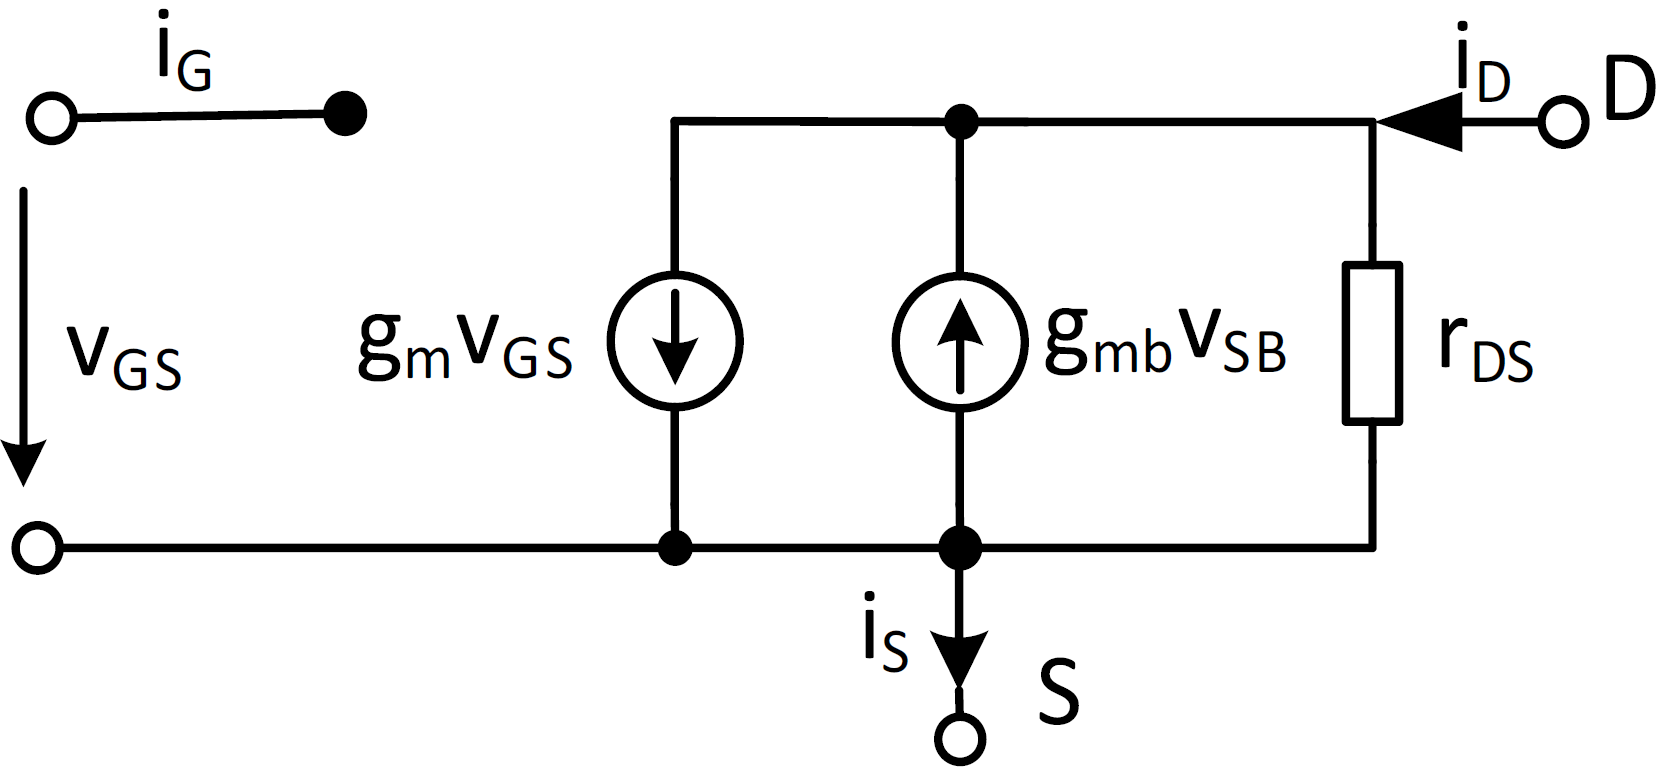
\includegraphics[width=\columnwidth, align=t]{images/02_MOSFET_Pi_Ersatzschaltung.png} Variante aus Skript
    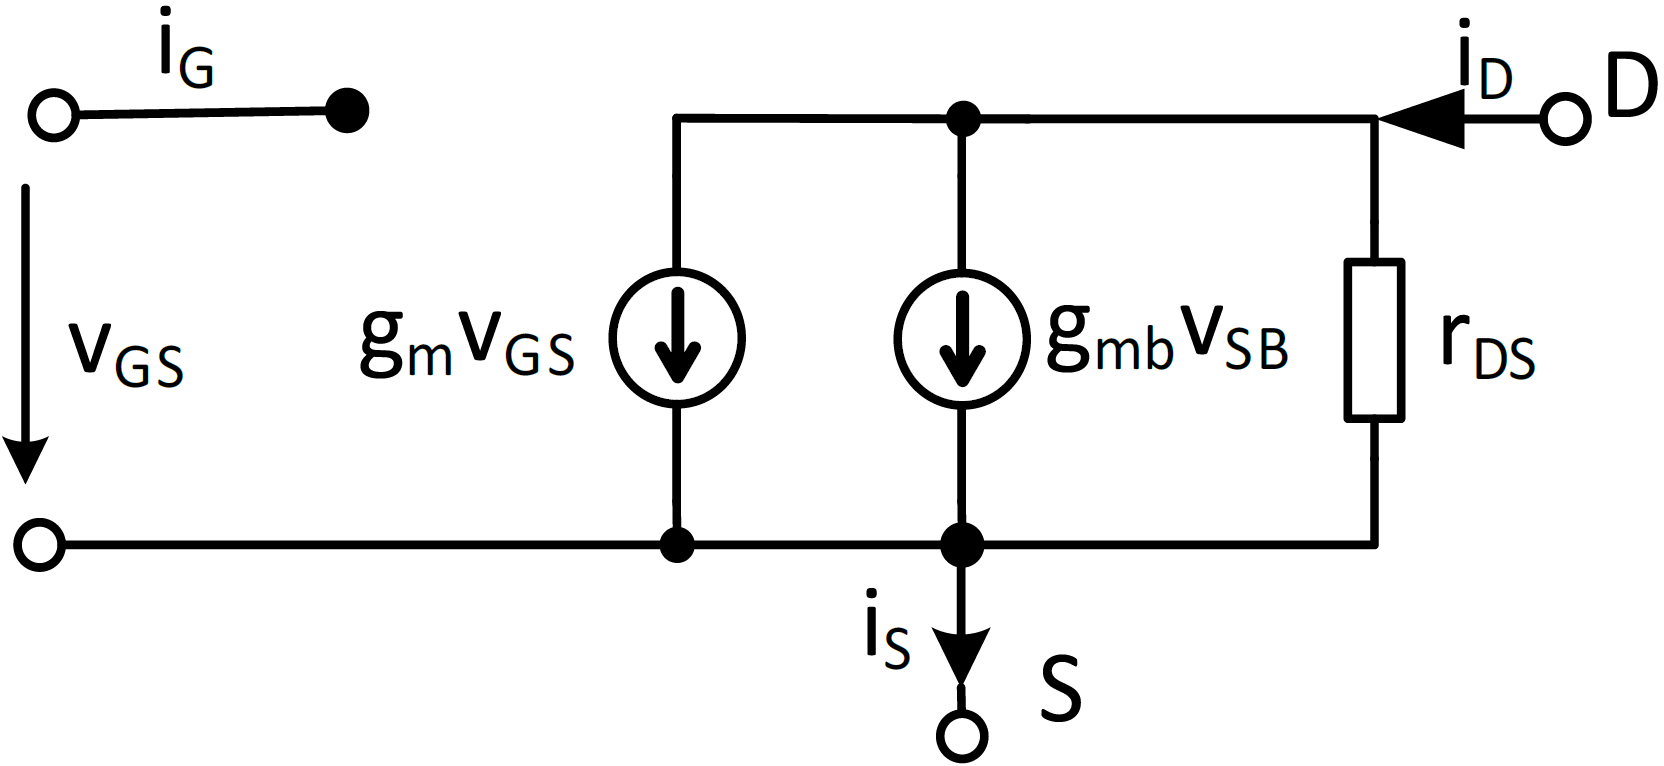
\includegraphics[width=\columnwidth, align=t]{images/02_MOSFET_Pi_Ersatzschaltung_angepasste_Stromrichtung.png}
\end{minipage}
\hfill
\begin{minipage}[t]{0.48\columnwidth}
    \raggedright
    \begin{itemize}
        \item Ideale spannungsgesteurte Stromquelle: $I_D = f(V_{GS})$
        \item Berücksichtigung von Kanallängenmodulation: $g_0$ bzw. $r_{DS}$
        \item Berücksichtigung von Body-Effekt: $g_{mb} \cdot V_{SB}$
    \end{itemize}
\end{minipage}


\paragraph{Hochfrequenz}
\label{Hochfrequenz}

\begin{minipage}[t]{0.48\columnwidth}
    % 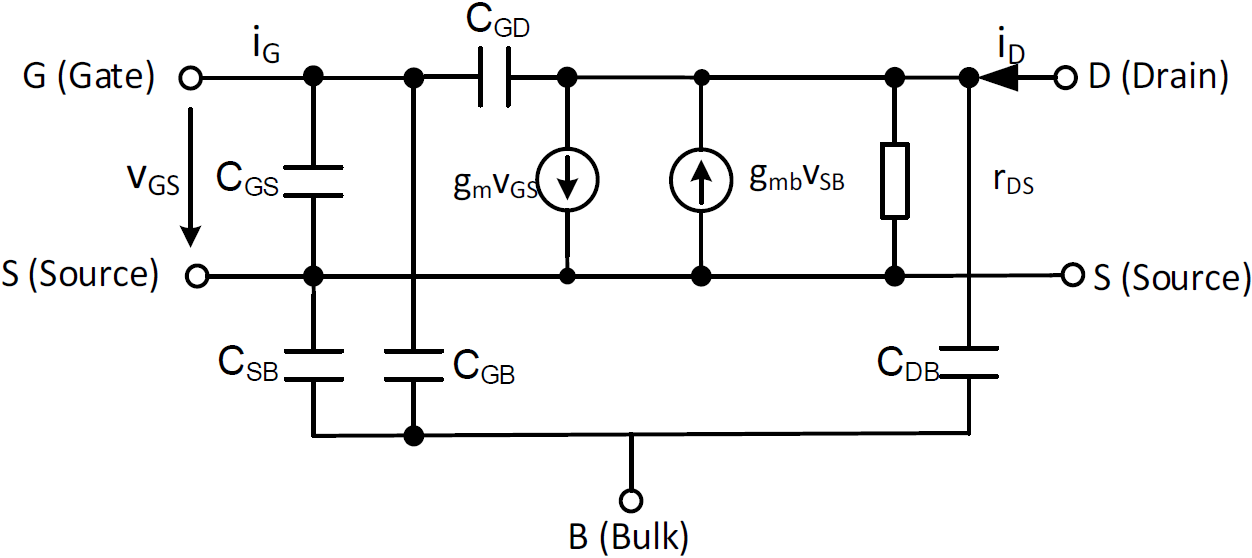
\includegraphics[width=\columnwidth, align=t]{images/02_MOSFET_Kleinsignalersatzschaltung_hochfrequent.png}   Variante aus Skript
    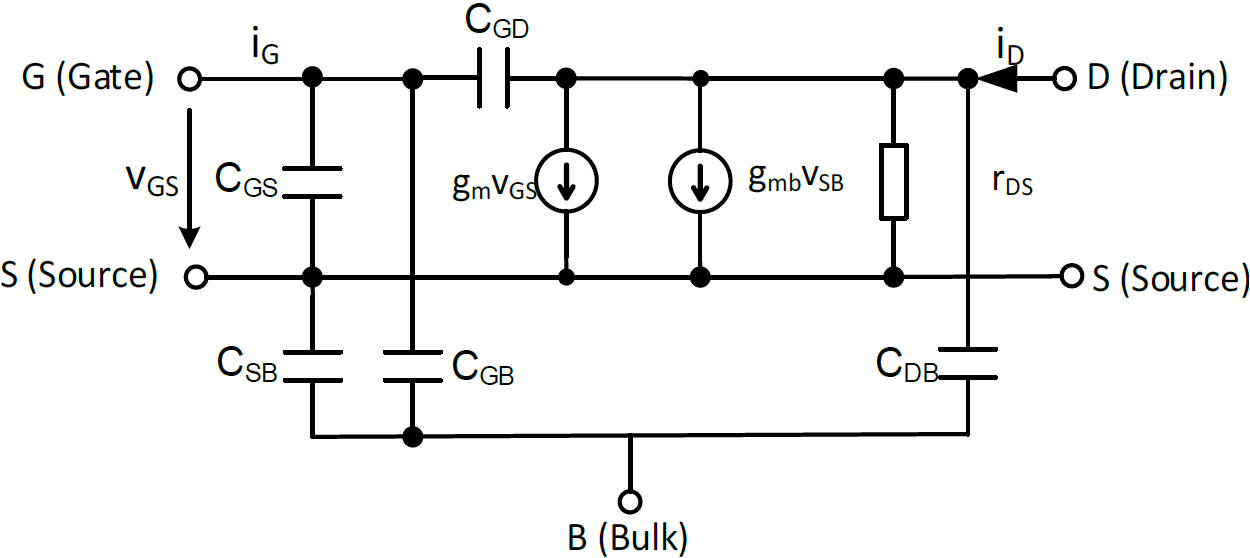
\includegraphics[width=\columnwidth, align=t]{images/02_MOSFET_Kleinsignalersatzschaltung_hochfrequent_angepasste_Stromrichtung.png}
\end{minipage}
\hfill
\begin{minipage}[t]{0.48\columnwidth}
    \raggedright
    Wenn Source und Bulk verbunden sind werden
    \begin{itemize}
        \item $C_{GB}$ und $C_{GS}$ parallel geschaltet und
        \item $C_{SB}$ kurzgeschlossen.
    \end{itemize}
\end{minipage}


\subsection{Kleinsignalparameter}
\label{Kleinsignalparameter}

Die Kleinsignalparameter bilden eine Vereinfachung (\textbf{Linearisierung}) in einem Arbeitspunkt. 
Sie berechnen sich daher allgemein folgendermassen aus der Ableitung
\[
    g_m          = \frac{\diff}{\diff V_{GS}} I_D \qquad
    g_0 = r_{DS} = \frac{\diff}{\diff V_{DS}} I_D \qquad
    g_{mb}       = \frac{\diff}{\diff V_{SB}} I_D
\]

Für die beiden Kanalzustände, in welchen Formeln für die Handrechnung verfügbar sind, gibt es auch hier handliche Formeln für die Berechnung der Kleinsignalparameter.

\smallskip

Die Bezeichnung der einzelnen Parameter gilt sowohl für strong inversion als auch für weak inversion.

\medskip

\begin{tabular}{@{}ll@{}}
    $g_m$               & Transkonduktanz (Stromquellenbetrieb) \textrightarrow\ Mass für Verstärkung des Transistors   \\
    $g_{mb}$            & Body-Transkonduktanz \textrightarrow\ Beschreibt Wirkung des Body-Effekts                     \\
    $g_0$               & Ausgangsleitwert (Stromquellenbetrieb) \textrightarrow\ beschreibt Kanallängenmodulation      \\
    $r_{DS \crd{0}}$    & Kleinstmöglicher Ausgangswiderstand bzw. \textbf{Einschaltwiderstand bei} $\bm{V_{DS} = 0}$   \\
                        & \textrightarrow\ Nur im Widerstandsbetrieb interessant
\end{tabular}

\medskip

\textbf{Hinweis:} Folgende Formel gelten für nMOS Transistoren.
Für pMOS Transistoren müssen jeweils \textbf{Beträge} eingesetzt werden \textbf{(ausser bei Technologieparametern)} und vor dem Gesamtresultat ein \textbf{Minus} ergänzt werden.


\subsubsection{Strong Inversion}

\vspace{-0.3cm}

\[
    \underbrace{ g_m = \mu C_{ox} \frac{W}{L} (V_{GS} - V_T) }_{\text{AP durch } V_{GS} \text{ bestimmt}} \qquad \qquad \qquad
    \underbrace{ g_m = \sqrt{2 \mu C_{ox} \frac{W}{L} I_D} }_{\text{AP durch } I_D \text{ bestimmt}} 
\]

% \[
%     g_{mb} = -g_m \frac{\gamma}{2 \sqrt{\abs{V_{SB}} + \abs{2 \Phi_F}}} = - g_m (n_M - 1)
% \]
% Ungesättigt:
% \[
%     g_0 = \frac{1}{r_{DS}} = \mu C_{ox} \frac{W}{L} ((V_{GS} - V_T) - V_{DS})
% \]
% % Gesättigt:
% \[
%     g_0 =  \frac{1}{r_{DS}} = \lambda I_{DS, sat} = \frac{I_D}{V_E + V_{DS}} \approx \frac{I_D}{a_E L + V_{DS}}
% \]

\vspace{-0.15cm}

\begin{align*}
                                         g_{mb} &= -g_m \frac{\gamma}{2 \sqrt{\abs{V_{SB}} + \abs{2 \Phi_F}}} = - g_m (n_M - 1)                                     \\
    \text{ \textbf{Ungesättigt:}} \quad     g_0 &= \frac{1}{r_{DS}} = \mu C_{ox} \frac{W}{L} ((V_{GS} - V_T) - V_{DS})                                              \\
    \text{ \textbf{Gesättigt:}} \quad       g_0 &=  \frac{1}{r_{DS}} = \lambda \cdot I_{DS, \rm sat} = \frac{I_D}{V_E + V_{DS}} \approx \frac{I_D}{a_E \cdot L + V_{DS}}
\end{align*}


\subsubsection{Weak Inversion}

\vspace{-0.3cm}

\[
    g_m = \frac{I_D}{n_M \cdot V_\text{temp}} \quad \text{ \textrightarrow\ Unabhängig von der Geometrie des Transistors!}
\]
% {
%     \raggedleft
%     \textrightarrow\ Unabhängig von der Geometrie des Transistors! \phantom{M}

% }

\vspace{-0.15cm}

\begin{align*}
                                         g_{mb} &= -g_m \frac{\gamma}{2 \sqrt{\abs{V_{SB}} + \abs{2 \Phi_F}}} = - g_m (n_M - 1)                                             \\
    \text{ \textbf{Ungesättigt:}} \quad     g_0 &= \frac{1}{r_{DS}} = \frac{V_{\text{temp}}}{I_{D \infty}} \quad \text{ \textrightarrow\ wird meist simuliert}              \\
    \text{ \textbf{Gesättigt:}} \quad       g_0 &=  \frac{1}{r_{DS}} = \lambda \cdot  I_{DS, \rm sat} = \frac{I_D}{V_E + V_{DS}}  \approx \frac{I_D}{a_E \cdot L + V_{DS}}
\end{align*}


% \[
%     g_{mb} = -g_m \frac{\gamma}{2 \sqrt{\abs{V_{SB}} + \abs{2 \Phi_F}}} = - g_m (n_M - 1)
% \]
% Ungesättigt:
% \[
%     g_0: \text{Wird üblicherweise simuliert}
% \]
% Gesättigt:
% \[
%     g_0 = \frac{1}{r_{DS}} = \lambda I_{DS, sat} = \frac{I_D}{V_E + V_{DS}}
% \]

\subsection{Zusammenhänge}
%TODO: [Flurin] This seems important but I don't know how to integrate this in a logical way
% [Simi] @Flurin: Leave it here for the moment... maybe we can fit in in somewhere late or we just leave it here :) 

$g_m$ ist in der Weak Inversion unabhängig der Geometrie. 
Es ist für einen gegebenen Drainstrom möglich, Transistoren, die in Weak Inversion wie auch welche, die in Strong Inversion sind herzustellen.
Das $g_m$ steigt beim Transistor in Strong Inversion 

\subsection{Bestimmung von Ersatzschaltbildern -- Allgemein}
\subsubsection{Grosssignalersatzschaltung}
\label{Grosssignalersatzschaltung}

Zur Bestimmung des \textbf{Arbeitspunkts} bzw.\ aller Gleichspannungen.
\begin{description}
    \item[AC-Spannungsquellen] durch Kurzschlüsse ersetzen.
    \item[AC-Stromquellen] durch Unterbrüche ersetzen. 
    \item[Kondensatoren] durch Unterbrüche ersetzen.
    \item[Spulen] durch Kurzschlüsse ersetzen.  
\end{description}

\subsubsection{Kleinsignalersatzschaltung}
\label{Kleinsignalersatzschaltung}
Zur Berechnung von Verstärkungsfaktoren und Eingangswiderständen für AC-Signale.

\begin{description}
    \item[DC-Spannungsquellen] durch Kurzschlüsse ersetzen.
    \item[DC-Stromquellen] durch Unterbrüche ersetzen. 
    \item[Nichtlineare Bauteile] durch deren Kleinsignalersatzschaltbild ersetzen.
    \item[Koppel- und Bypass-Kondensatoren] durch Kurzschlüsse ersetzen.  
\end{description}


\subsection{Vorgehen: Verstärker dimensionieren}
\begin{itemize}
    \item Arbeitspunkt bestimmen.
    \item $I_D$ wählen, sodass der Transistor \textbf{gesättigt} ist.   %CHECK [Simi] @Flurin Hier stand zuvor UNgesättigt -> gemäss Beispiel von V4 S15 haben wir aber gesagt, der Transistor muss gesättigt sein...?
    \item Kleinsignalersatzschaltung zeichnen.
    \item Parameter der Ersatzschaltung bestimmen.
\end{itemize}